\documentclass[aspectratio=169, handout]{beamer}
\usepackage{will_handley}

% Commands
% --------
% - \arxiv{arxiv number}
% - \cols{width}{lh column}{rh column}
% -  \begin{fig(left|right)}[fractional width (e.g 0.6) ]{name of image}
%        content of other column
%    \end{fig(left|right)}

% Talk details
% ------------
\title{Next generation cosmological analysis with nested sampling}
\date{8\textsuperscript{th} September 2022}
\newcommand{\av}[2][]{\left\langle #2\right\rangle_{#1}}

\begin{document}

\begin{frame}
    \titlepage
\end{frame}

\begin{frame}
    \frametitle{Summary}
\end{frame}

\begin{frame}
    \frametitle{The three pillars of Bayesian inference}
    \begin{itemize}
        \item Parameter estimation: ``What do the data tell me about my model?'':
            \[ \C[0]{P(\theta|D,M)} = \frac{\C[2]{P(D|\theta,M)} \C[1]{P(\theta|M)}}{\C[3]{P(D|M)}}, \qquad \C[0]{\mathcal{P}} = \frac{\C[2]{\mathcal{L}} \times\C[1]{\pi}}{\C[3]{\mathcal{Z}}}, \qquad \C[0]{\text{Posterior}} = \frac{\C[2]{\text{Likelihood}} \times\C[1]{\text{Prior}}}{\C[3]{\text{Evidence}}}. \]
        \item Model comparison: ``Which model best fits the data?'':
            \[ \C[4]{P(M|D)} = \frac{\C[3]{P(D|M)} \C[5]{P(M)}}{\C[6]{P(D)}}, \qquad \frac{\C[3]{\mathcal{Z}_\mathcal{M}} \C[5]{\Pi_\mathcal{M}}}{\C[6]{\sum_m Z_m \Pi_m}}, \qquad \C[4]{\text{Model Posterior}} = \frac{\C[3]{\text{Evidence}} \times\C[5]{\text{Model Prior}}}{\C[6]{\text{Normalisation}}}.\]
        \item Tension quantification: ``Are datasets consistent within a given model?'' \arxiv{1902.04029}
        \[ \mathcal{R} = \frac{\mathcal{Z}_{AB}}{\mathcal{Z}_A\mathcal{Z}_\mathcal{B}}, \qquad \log\mathcal{S} = \av[\mathcal{P}_{AB}]{\log\mathcal{L}_{AB}}-\av[\mathcal{P}_{A}]{\log\mathcal{L}_{B}}-\av[\mathcal{P}_{B}]{\log\mathcal{L}_{B}}  \]
    \end{itemize}
\end{frame}

\begin{frame}
    \frametitle{Occam's Razor~\arxiv{2102.11511}}
    \begin{itemize}
        \item Bayesian inference quantifies Occam's Razor:
            \begin{itemize}
                \item \textit{``Entities are not to be multiplied without necessity''} \hfill --- William of Occam
                \item \textit{``Everything should be kept as simple as possible, but not simpler''} \hfill --- ``Albert Einstein''
            \end{itemize}
        %\item Consider the Evidence $\C[3]{\mathcal{Z}\equiv P(D|M)}$: 
        %    \begin{description}[Parameter estimation]
        %        \item [Parameter estimation] normalisation constant
        %        \item [Model comparison] critical update factor for \C[5]{model prior} to \C[4]{model posterior}
        %    \end{description}
        \item Properties of the evidence: rearrange Bayes' theorem for parameter estimation
            \[\C[0]{\mathcal{P}(\theta)} = \frac{\C[2]{\mathcal{L}(\theta)} \C[1]{\pi(\theta)}}{\C[3]{\mathcal{Z}}} \qquad\Rightarrow\qquad \C[3]{\log \mathcal{Z}} = \C[2]{\log\mathcal{L}(\theta)} - \log \frac{\C[0]{\mathcal{P}(\theta)}}{\C[1]{\pi(\theta)}} \]  
        \item Evidence is composed of a ``goodness of fit'' term  and ``Occam Penalty''
    \end{itemize}
    \begin{columns}[t]
        \column{0.5\textwidth}
    \begin{itemize}
        \item RHS true for all $\theta$. Take max likelihood value $\theta_*$:
            \[
                \C[3]{\log \mathcal{Z}} = -\chi_\mathrm{min}^2 - \text{Mackay penalty}
            \]
    \end{itemize}
        \column{0.5\textwidth}
    \begin{itemize}
        \item Be more Bayesian and take posterior average to get the ``Occam's razor equation''
            \[
                \boxed{
                    \C[3]{\log \mathcal{Z}} = \av[{\C[0]{\mathcal{P}}}]{\C[2]{\log\mathcal{L}}} - \mathcal{D}_\mathrm{KL}
            }
            \]
    \end{itemize}
    \end{columns}
    \vfill
    \begin{itemize}
        \item Natural regularisation which penalises models with too many parameters.
    \end{itemize}
\end{frame}

\begin{frame}
    \frametitle{Kullback Liebler divergence}
    \begin{columns}
        \column{0.5\textwidth}
        \begin{itemize}
            \item The KL divergence between \C[1]{prior $\pi$} and \C[0]{posterior $\mathcal{P}$} is is defined as:
                \[\mathcal{D}_\mathrm{KL} = \av[\mathcal{P}]{\log\frac{\mathcal{P}}{\pi}} = \int \mathcal{P}(\theta) \log \frac{\mathcal{P}(\theta)}{\pi(\theta)}d\theta.\]
            \item Whilst not a distance, $\mathcal{D}=0$ when $\mathcal{P}=\pi$.
            \item Occurs in the context of machine learning as an objective function for training functions.
            \item In Bayesian inference it can be understood as a log-ratio of ``volumes'':
                \[ \mathcal{D}_\mathrm{KL} \approx \log \frac{V_\pi}{V_\mathrm{P}}.\]
                (this is exact for top-hat distributions).
        \end{itemize}
        \column{0.5\textwidth}
        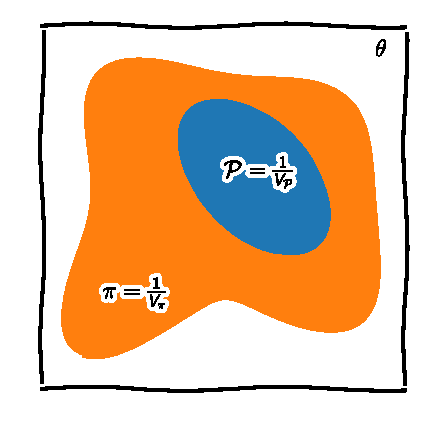
\includegraphics{figures/volumes.pdf}
    \end{columns}
\end{frame}

\begin{frame}
    \frametitle{Why do sampling?}
    \begin{columns}
        \column{0.5\textwidth}
        \begin{itemize}
            \item The cornerstone of numerical Bayesian inference is working with \C[3]{samples}.
            \item Generate a set of representative parameters drawn in proportion to the posterior $\theta\sim\mathcal{P}$.
            \item The magic of marginalisation $\Rightarrow$ perform usual analysis on each sample in turn.
            \item The golden rule is \C[1]{stay in samples} until the last moment before computing summary statistics/triangle plots because \[\boxed{f(\:\av{X}\:)\ne \av{\:f(X)\:}}\]
            \item Generally need $\sim\mathcal{O}(12)$ independent samples to compute a value and error bar.
        \end{itemize}
        \column{0.5\textwidth}
        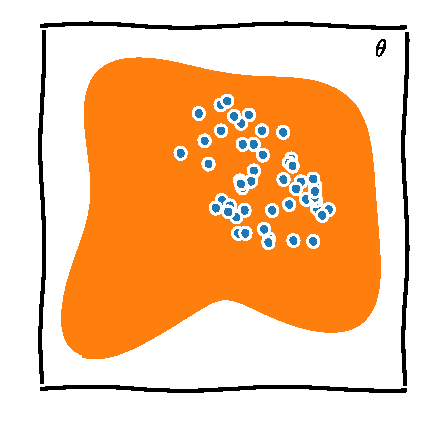
\includegraphics{figures/samples.pdf}
    \end{columns}
\end{frame}

\begin{frame}
    \frametitle{The importance of global measures of tension}
    \begin{columns}
        \begin{column}{0.5\textwidth}
            \begin{itemize}
                \item Hubble tension~\arxiv{1907.10625}
                    \begin{itemize}
                        \item \textit{Planck}: $H_0=67.4\pm0.5$
                        \item S$H_0$ES: $H_0=74.0\pm1.4$
                    \end{itemize}
                \item In other situations the discrepancy doesn't exist in a single interpretable parameter
                \item For example: DES+\textit{Planck} \arxiv{1902.04029} 
                \item Are these two datasets in tension?
                \item There are a lot more parameters -- are we sure that tensions aren't hiding? Are we sure we've chosen the best ones to reveal the tension?
                \item Should use ``Suspiciousness'' statistic $\mathcal{S}$, or Bayes ratio $\mathcal{R}$ to determine global tension.
            \end{itemize}
        \end{column}
        \begin{column}{0.5\textwidth}
            \includegraphics<1>{figures/DES_planck_1}
            \includegraphics<2>{figures/DES_planck_2}
        \end{column}
    \end{columns}
\end{frame}

\begin{frame}
    \frametitle{Suspiciousness statistic}
\end{frame}

\begin{frame}
    \frametitle{\texttt{unimpeded}}
    \texttt{anesthetic}
\end{frame}


\begin{frame}
    \frametitle{What is Nested Sampling?}
    \begin{itemize}
        \item Nested sampling is a multi-purpose numerical mathematical tool.
        \item Given a (scalar) function $f$ with a vector of parameters $\theta$, it can be used for:
    \end{itemize}
    \vspace{-10pt}
    \begin{columns}[t]
        \column{0.33\textwidth}
        \begin{block}{Optimisation}
            \vspace{-5pt}
            \[\theta_\mathrm{max} = \max_\theta{f(\theta)}\]
        \end{block}
        \column{0.33\textwidth}
        \begin{block}{Sampling}
            \vspace{-5pt}
            \[\text{draw }\theta\sim f\]
        \end{block}
        \column{0.33\textwidth}
        \begin{block}{Integration}
            \vspace{-5pt}
            \[\int f(\theta) dV \]
            \vspace{-15pt}
        \end{block}
    \end{columns}
    \begin{columns}[t]
        \column{0.33\textwidth}
        \centerline{\includegraphics[width=0.8\textwidth,page=13]{figures/himmelblau}}
        \column{0.33\textwidth}
        \centerline{\includegraphics[width=0.8\textwidth,page=15]{figures/himmelblau}}
        \column{0.33\textwidth}
        \centerline{\includegraphics[width=0.8\textwidth,page=14]{figures/himmelblau}}
    \end{columns}
\end{frame}

\begin{frame}
    \frametitle{MCMC sampling}
    \begin{columns}
        \column{0.6\textwidth}
        \begin{itemize}
            \item Markov chain based methods generate samples from posterior distribution by a stepping procedure.
            \item This can get stuck in local peaks.
            \item Cannot compute normalisation $\mathcal{Z}$ of Bayes theorem:
                \[ \C[0]{P(\theta|D,M)} = \frac{\C[2]{P(D|\theta,M)}\C[1]{P(\theta|M)}}{\C[3]{P(D|M)}},\]
                \[ \C[0]{\mathcal{P}} = \frac{\C[2]{\mathcal{L}}\times \C[1]{\pi}}{\C[3]{\mathcal{Z}}}, \qquad \C[0]{\text{posterior}} = \frac{\C[2]{\text{likelihood}}\times \C[1]{\text{prior}}}{\C[3]{\text{evidence}}}. \]
            \item We generally want the evidence $\C[3]{\mathcal{Z}=P(D|M)}$ for the second stage of inference: model comparison:
                \[ P(M|D) = \frac{\C[3]{P(D|M)}P(M)}{P(D)}, \qquad \text{Science}(M) = \frac{\C[3]{\mathcal{Z}_M} \Pi_M}{\sum_m \C[3]{\mathcal{Z}}_m \Pi_m}. \]

        \end{itemize}
        \column{0.4\textwidth}

        \includegraphics<1>[width=\textwidth,page=16]{figures/himmelblau}%
        \includegraphics<2>[width=\textwidth,page=17]{figures/himmelblau}%
        \includegraphics<3>[width=\textwidth,page=18]{figures/himmelblau}%
        \includegraphics<4>[width=\textwidth,page=19]{figures/himmelblau}%
        \includegraphics<5>[width=\textwidth,page=20]{figures/himmelblau}%
        \includegraphics<6>[width=\textwidth,page=21]{figures/himmelblau}%

    \end{columns}
\end{frame}

\begin{frame}
    \frametitle{Nested sampling}
    \begin{columns}
        \column{0.6\textwidth}
        \begin{itemize}
            \item Nested sampling: completely different way to sample.
            \item Ensemble sampling to compress prior to posterior.
            \item Sequentially update a set $S$ of $n$ samples:
                \begin{itemize}
                    \item[$S_0$:]  Generate $n$ samples uniformly over the space (from the prior $\pi$). 

                    \item[$S_{i+1}$:] Delete the lowest likelihood sample in $S_{i}$, and replace it with a new uniform sample with higher likelihood.
                \end{itemize}
            \item Requires one to be able to sample uniformly within a region, subject to a {\em hard likelihood constraint}:
                \[\{\theta\sim \pi : \mathcal{L}(\theta)>\mathcal{L}_*. \}\]
            \item This procedure optimises (multimodally), and can calculate the \C[3]{evidence} \& \C[0]{posterior} weights.
        \end{itemize}
        \column{0.4\textwidth}

        \includegraphics<1|handout:0>[width=\textwidth,page=1]{figures/himmelblau}%
        \includegraphics<2|handout:0>[width=\textwidth,page=2]{figures/himmelblau}%
        \includegraphics<3|handout:0>[width=\textwidth,page=3]{figures/himmelblau}%
        \includegraphics<4          >[width=\textwidth,page=4]{figures/himmelblau}%
        \includegraphics<5|handout:0>[width=\textwidth,page=5]{figures/himmelblau}%
        \includegraphics<6|handout:0>[width=\textwidth,page=6]{figures/himmelblau}%
        \includegraphics<7|handout:0>[width=\textwidth,page=7]{figures/himmelblau}%
        \includegraphics<8|handout:0>[width=\textwidth,page=8]{figures/himmelblau}%

    \end{columns}
\end{frame}

\begin{frame}
    \frametitle{Mathematics of Nested Sampling}
    \framesubtitle{A probabilistic Lebesgque integrator}
    \begin{columns}
        \column{0.5\textwidth}
        \begin{itemize}
            \item At each iteration, the likelihood contour will shrink in volume by  $\approx 1/n$.
            \item Nested sampling zooms in to the peak of the function $\mathcal{L}$ {\em exponentially}.
                \vspace{-5pt}
                \[
                    \mathcal{Z} \approx \sum_i \Delta\mathcal{L}_i X_{i}, \quad
                    X_{i+1} \approx \frac{n}{n+1}X_i, \quad X_{0} = 1 .
                \]
                \vspace{-15pt}
            \item Although this is only approximate, we can quantify the error 
                \vspace{-10pt}
                \[
                    P(X_i|X_{i-1}) = \frac{X_{i}^{n-1}}{nX_{i-1}^n}\times[0<X_i<X_{i-1}].
                \]
                \vspace{-15pt}
            \item Integral can be discretised in several ways
                \vspace{-10pt}
                \[
                    \mathcal{Z} \approx \sum_i \Delta\mathcal{L}_i X_{i} = \sum_i \mathcal{L}_i \Delta X_{i} = \sum_i \tfrac{\mathcal{L}_i+\mathcal{L}_{i-1}}{2}{\small(X_{i-1}-X_i).}
                \]

        \end{itemize}
        \column{0.5\textwidth}
        \includegraphics<1|handout:0>[width=\textwidth,page=1]{figures/lesbesgue}%
        \includegraphics<2|handout:0>[width=\textwidth,page=2]{figures/lesbesgue}%
        \includegraphics<3|handout:0>[width=\textwidth,page=3]{figures/lesbesgue}%
        \includegraphics<4|handout:0>[width=\textwidth,page=4]{figures/lesbesgue}%
        \includegraphics<5|handout:0>[width=\textwidth,page=5]{figures/lesbesgue}%
        \includegraphics<6|handout:0>[width=\textwidth,page=6]{figures/lesbesgue}%
        \includegraphics<7|handout:0>[width=\textwidth,page=7]{figures/lesbesgue}%
        \includegraphics<8|handout:0>[width=\textwidth,page=8]{figures/lesbesgue}%
        \includegraphics<9|handout:0>[width=\textwidth,page=9]{figures/lesbesgue}%
        \includegraphics<10|handout:0>[width=\textwidth,page=10]{figures/lesbesgue}%
        \includegraphics<11|handout:0>[width=\textwidth,page=11]{figures/lesbesgue}%
        \includegraphics<12|handout:0>[width=\textwidth,page=12]{figures/lesbesgue}%
        \includegraphics<13|handout:0>[width=\textwidth,page=13]{figures/lesbesgue}%
        \includegraphics<14|handout:0>[width=\textwidth,page=14]{figures/lesbesgue}%
        \includegraphics<15|handout:0>[width=\textwidth,page=15]{figures/lesbesgue}%
        \includegraphics<16          >[width=\textwidth,page=16]{figures/lesbesgue}%
    \end{columns}
\end{frame}

\begin{frame}
    \frametitle{Dead points: posteriors \& evidences}
    \begin{columns}
        \column{0.6\textwidth}
        \begin{itemize}
            \item At the end, one is left with a set of discarded points.
            \item These may be weighted to form weighted posterior samples using $w_i = \mathcal{L}_i \Delta X_i$.
            \item They can also be used to calculate the normalisation $\mathcal{Z} = \sum \mathcal{L}_i \Delta X_i$, or more generally $\sum_i f(\mathcal{L}_i) \Delta X_i$.
                \begin{itemize}
                    \item Nested sampling probabilistically estimates the volume of the parameter space
                        \[X_i \approx {\left(\frac{n}{n+1}\right)} X_{i-1} \quad\Rightarrow\quad
                        X_i \approx {\left(\frac{n}{n+1}\right)}^i \approx e^{-i/n}, \]
                    \item Nested sampling thus estimates the density of states,
                    \item it is therefore a partition function calculator
                        $Z(\beta) = \sum_i \mathcal{L}_i^\beta \Delta X_i$.
                \end{itemize}
            \item The evolving ensemble of live points allows algorithms to perform self-tuning and mode clustering.
        \end{itemize}

        \column{0.4\textwidth}

        \includegraphics<1|handout:0>[width=\textwidth,page=14]{figures/himmelblau}%
        \includegraphics<2          >[width=\textwidth,page=15]{figures/himmelblau}%

    \end{columns}

\end{frame}

\begin{frame}
  \frametitle{Sampling from a hard likelihood constraint} 
  
  \begin{quote}
    ``It is not the purpose of this introductory paper to develop the technology of navigation within such a volume. We merely note that exploring a hard-edged likelihood-constrained domain should prove to be neither more nor less demanding than exploring a likelihood-weighted space.''
    
   {\hfill --- John Skilling}
  \end{quote}

  \begin{itemize}
      
    \item A large fraction of the work in NS to date has been in attempting to implement a hard-edged sampler in the NS meta-algorithm $\{\theta\sim \pi : \mathcal{L}(\theta)>\mathcal{L}_* \}$.
    \item \url{https://projecteuclid.org/euclid.ba/1340370944}.
    \item There has also been much work beyond this (focus of this talk).
  \end{itemize}
 
\end{frame}


\begin{frame}
    \frametitle{Implementations of Nested Sampling}
    %\begin{columns}
    %    \begin{column}{0.33}
    %        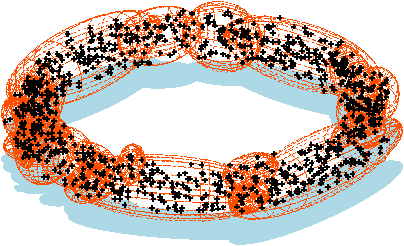
\includegraphics[width=\textwidth]{figures/multinest}
    %    \end{column} 
    %\end{columns}
    \begin{columns}[t]
        \column{0.3\textwidth}
        \texttt{MultiNest}~\arxiv{0809.3437}
        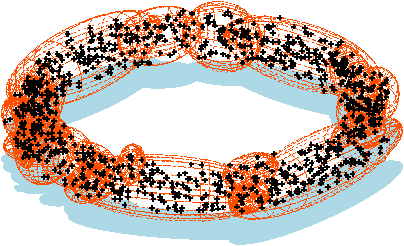
\includegraphics[width=\textwidth]{figures/multinest}
        \texttt{UltraNest}~\arxiv{2101.09604}
        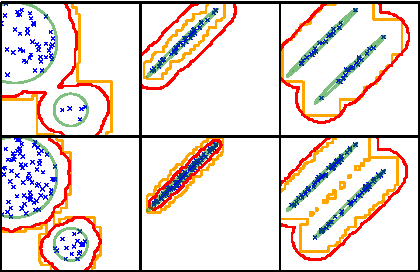
\includegraphics[width=\textwidth]{figures/radfriends}
        \column{0.4\textwidth}
        \texttt{PolyChord}~\arxiv{1506.00171}
        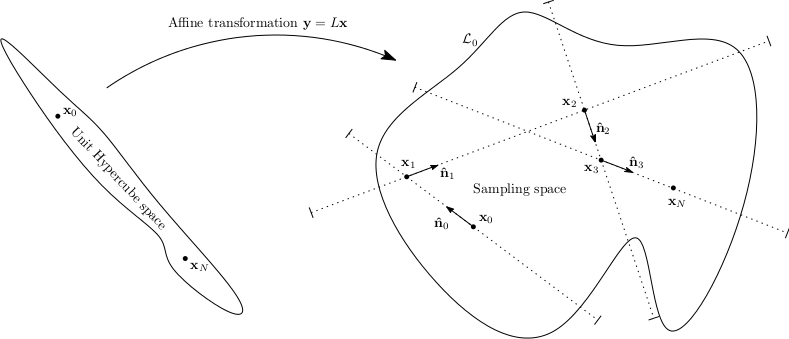
\includegraphics[width=\textwidth]{figures/polychord}
        \vfill
        \texttt{NeuralNest}~\arxiv{1903.10860}
        \begin{columns}
            \column{0.5\textwidth}
            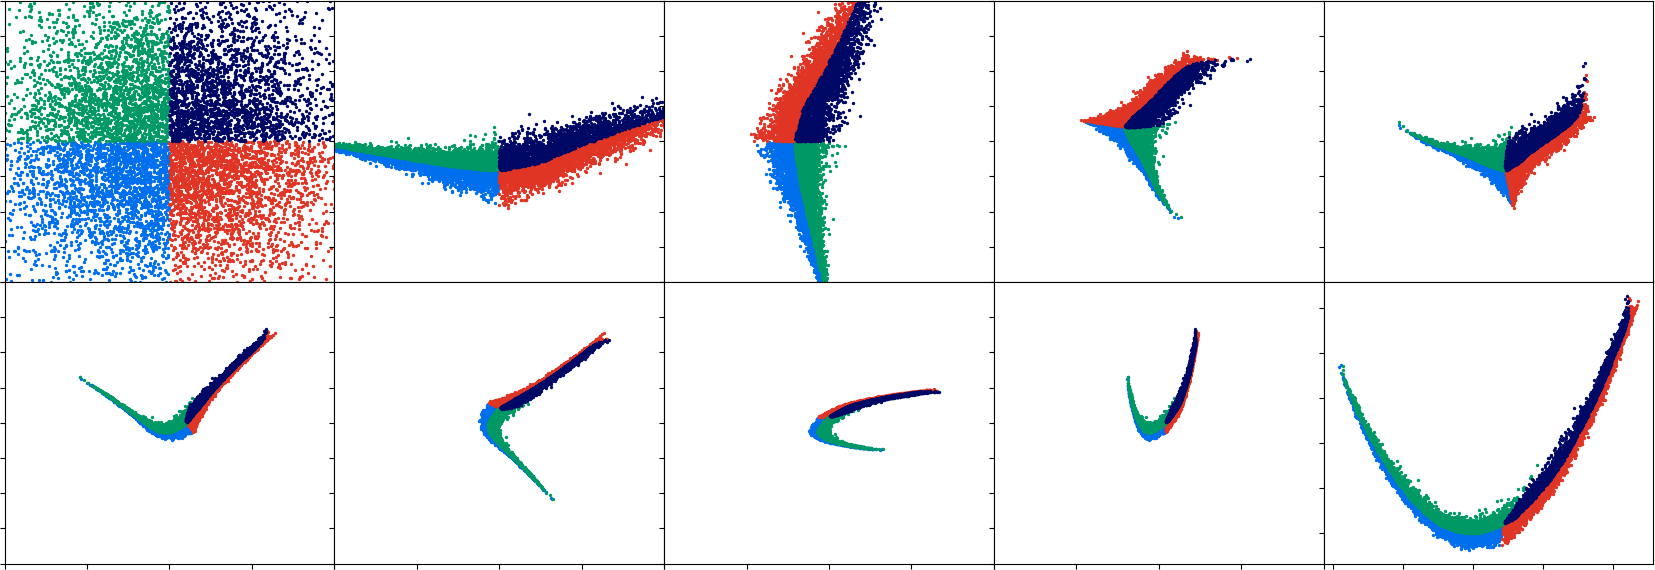
\includegraphics[width=\textwidth]{figures/rosenbrock_flow.png}
            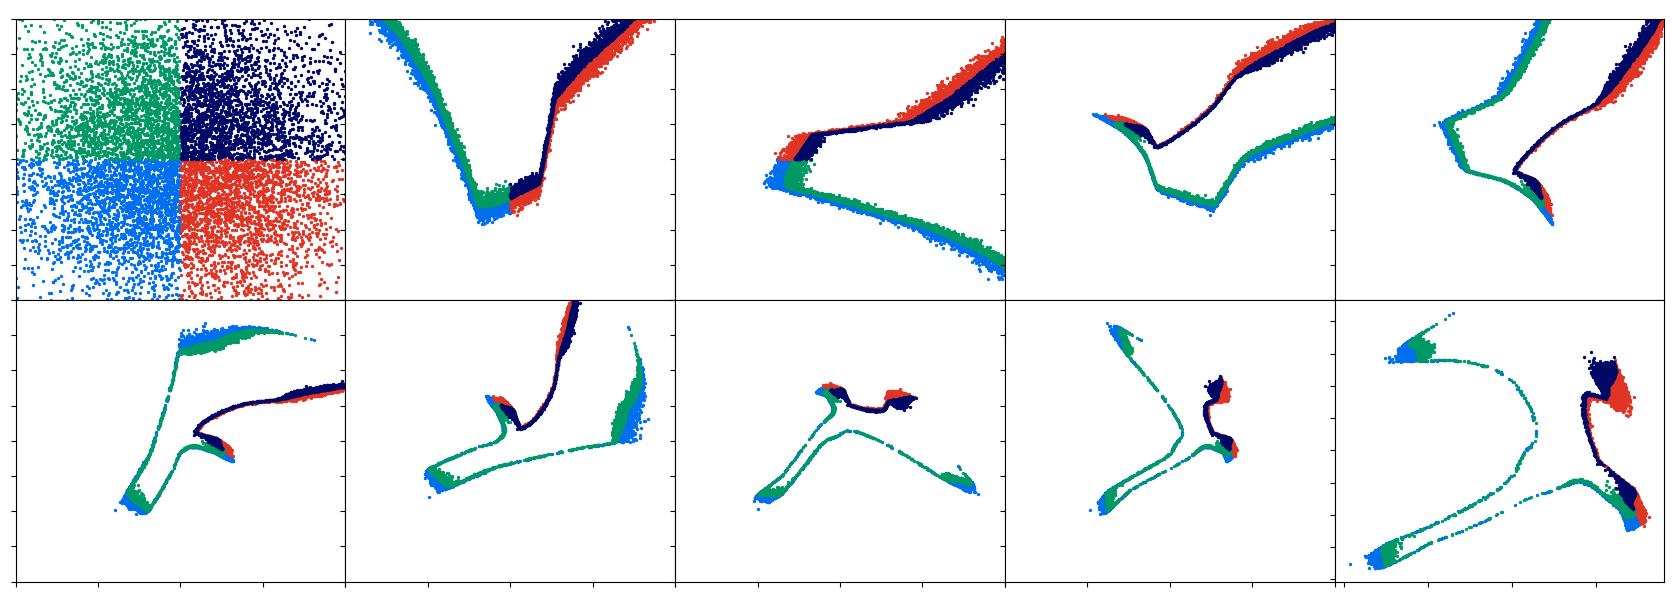
\includegraphics[width=\textwidth]{figures/himmelblau_flow.png}
            \column{0.5\textwidth}
            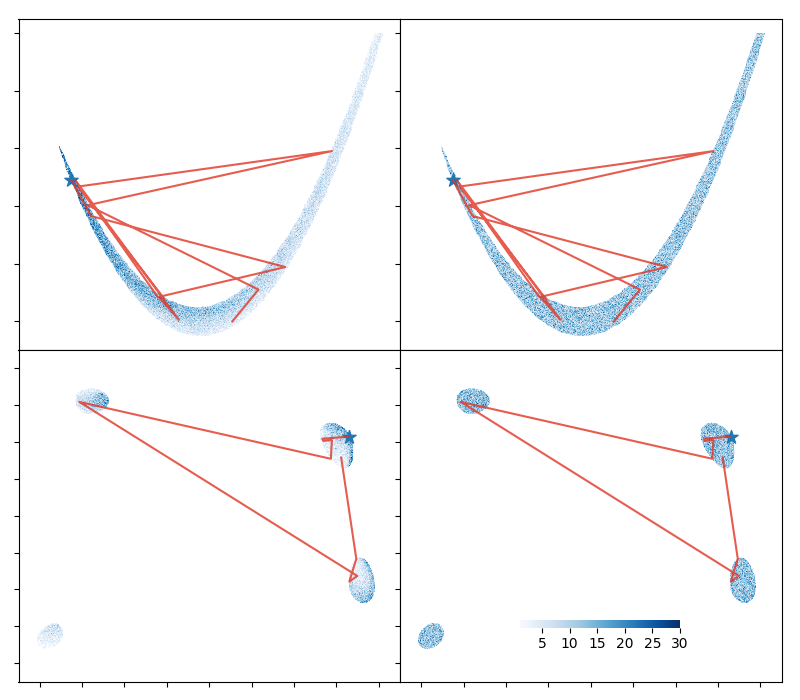
\includegraphics[width=\textwidth]{figures/chains.png}
        \end{columns}
        \texttt{dynesty}~\arxiv{1904.02180}
        \vfill
        \column{0.3\textwidth}
        \texttt{DNest}~\arxiv{1606.03757}
        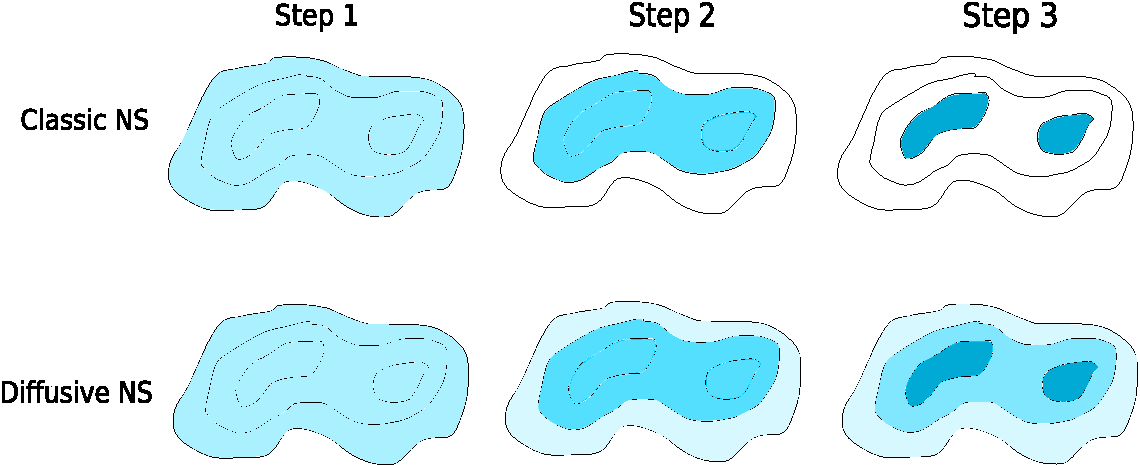
\includegraphics[width=\textwidth]{figures/dnest}
        \texttt{ProxNest}~\arxiv{2106.03646}
        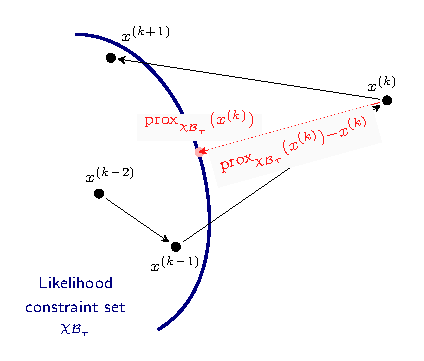
\includegraphics[width=\textwidth]{figures/proxnest_diagram}
        \vfill
    \end{columns}
\end{frame}

\begin{frame}
    \frametitle{The DES evidence ratio $R$}
    \begin{itemize}
        \item The Dark Energy Survey (\arxiv{1708.01530}) quantifies tension between two datasets $A$ and $B$ using the Bayes ratio:
            \[
                R = \frac{\mathcal{Z}_{AB}}{\mathcal{Z}_A \mathcal{Z}_B}
            \]
            where $\mathcal{Z}$ is the Bayesian evidence.
        \item Many attractive properties:
            \begin{itemize}
                \item Symmetry
                \item Parameterisation independence
                \item Dimensional consistency
                \item Use of well-defined Bayesian quantities
            \end{itemize}
        \item What does it mean?
    \end{itemize}
\end{frame}

\begin{frame}
    \frametitle{Bayesian evidence $\mathcal{Z}$}
    \begin{itemize}
        \item Bayes theorem for parameter estimation:
    \[
    P(\theta|D) = \frac{P(D|\theta)P(\theta)}{P(D)} \quad\longrightarrow\quad \text{Posterior} = \frac{\text{Likelihood}\times\text{Prior}}{\text{Evidence}}
    \]
        \item Normalising constant $\equiv$ Bayesian evidence $\equiv$ $P(D)$ is hard to compute:
    \[
        P(D) = \int P(D|\theta)P(\theta) d\theta = \left\langle \text{Likelihood} \right\rangle_\text{Prior}
    \]
        \item Traditionally used to compare models using the same data
        \item For DES, it is used to compare different data with the same model.
        \item Computed using nested sampling (\texttt{MultiNest}, \texttt{PolyChord}, \texttt{dynesty}), simulated annealing (\texttt{emcee}), or from MCMC using \texttt{MCEvidence}.
    \end{itemize}
\end{frame}

\begin{frame}
    \frametitle{Bayesian evidence $\mathcal{Z}$: Prior dependency}
    \begin{itemize}
        \item Bayesian evidences are prior dependent:
            \[
                \mathcal{Z} = \int P(D|\theta)P(\theta) d\theta \approx \langle\text{Likelihood}\rangle_\text{Posterior} \times \frac{\text{Posterior volume}}{\text{Prior volume}}
            \]
        \item They balance ``goodness of fit'' via likelihood with ``complexity'' through Occam penalty.
        \item Models that include too many fine-tuned parameters are disfavoured, unless they provide a much better fit.
        \item Corollary: Unconstrained parameters are not penalised.
        \item Widen prior $\Rightarrow$ reduce evidence \\ (providing prior does not cut into posterior).
        \item Bayesians vs Frequentists $\leftrightarrow$ Feature vs Bug.
    \end{itemize}
\end{frame}


\begin{frame}
    \frametitle{The meaning of the DES evidence ratio $R$}
    \begin{itemize}
        \item The Dark Energy Survey collaboration (\arxiv{1708.01530}) quantify tension between two datasets $A$ and $B$ using the Bayes ratio:
            \[
                R = \frac{\mathcal{Z}_{AB}}{\mathcal{Z}_A \mathcal{Z}_B} = \frac{P(A\cap B)}{P(A)P(B)} = \frac{P(A|B)}{P(A)} = \frac{P(B|A)}{P(B)}
            \]
        \item $R$ gives the relative change in our confidence in data $A$ in light of having seen $B$ (and vice-versa).
        \item $R>1$ implies we have more confidence in $A$ having received $B$.
        \item Like evidences, it is prior-dependent
        \item Increasing prior widths $\Rightarrow$ increasing confidence.
    \end{itemize}
\end{frame}

\begin{frame}
    \frametitle{The DES evidence ratio $R$: Prior dependency}
    {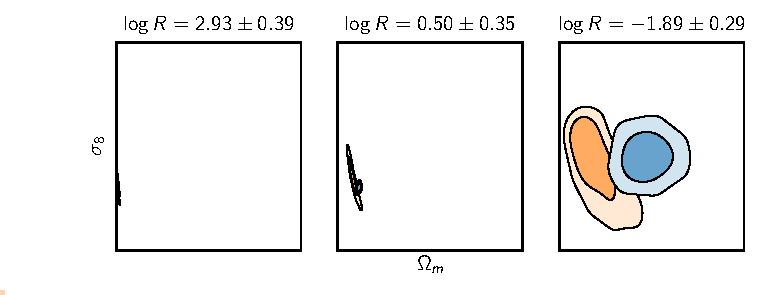
\includegraphics[trim=0.6in 0.3in 0in 0in]{./plots/prior_dependency.pdf}}
    \begin{itemize}
        \item What does it mean if increasing prior widths $\Rightarrow$ increasing confidence? 
        \item Wide priors mean {\em a-priori\/} the parameters could land anywhere.
        \item We should be proportionally more reassured when they land close to one another if the priors are wide
    \end{itemize}
\end{frame}

\begin{frame}
    \frametitle{How do we deal with the prior dependency in $R$?}
    \begin{description}
        \item[Option 1] Take the Bayesian route, accept the prior dependency, and spend time trying to justify why a given set of priors are ``physical''.
        \item[Option 2] Try to find a principled way of removing this prior dependency
    \end{description}
    \begin{itemize}
        \item One of the critical observations is that one can only hide tension by widening priors. Narrowing them will only ever show tension if it is present.
        \item If we could define ``Narrowest reasonable priors'' and find that $R<1$, then this would indicate tension.
    \end{itemize}
\end{frame}

\begin{frame}
    \frametitle{$R$: a Gaussian example}
    \begin{itemize}
        \item Given two Gaussians with parameter means $\mu_A,\mu_B$ and parameter covariances $\Sigma_A,\Sigma_B$ and a prior with volume $V_\pi$:
            \begin{align}
                \log R =& -\frac{1}{2} (\mu_A-\mu_B){(\Sigma_{A}+\Sigma_{B})}^{-1}(\mu_A-\mu_B)\nonumber\\
                & + \log V_\pi\nonumber -\log\sqrt{|2\pi(\Sigma_{A}+\Sigma_{B})|} 
            \end{align}
        \item Like evidence, $R$ composed of ``Goodness of fit'', and ``Occam factor''.
        \item Ideally want would remove this Occam factor (ratio of prior to posterior volume).
    \end{itemize}
\end{frame}

\begin{frame}
    \frametitle{KL divergence $\mathcal{D}$, Information $\mathcal{I}$, suspiciousness $S$}
    \begin{itemize}
        \item The KL divergence quantifies the compression from prior to posterior:
            \[
                \mathcal{D} = \int P(\theta|D) \log \frac{P(\theta|D)}{P(\theta)} d\theta = \left\langle\log\frac{\text{Posterior}}{\text{Prior}}\right\rangle_\text{Posterior}
            \]
        \item It bears many similarities to an Occam factor, for a Gaussian:
            \[
                \mathcal{D} =   \log V_\pi - \log \sqrt{|2\pi\Sigma|} - \frac{1}{2}d
            \]
        \item Can define equivalent of $R$ for KL divergence, the information ratio $\mathcal{I}$
            \begin{align}
                \log R &= \mathcal{Z}_{AB} -\mathcal{Z}_A - \mathcal{Z}_B \nonumber\\
                \log \mathcal{I} &= \mathcal{D}_A + \mathcal{D}_B - \mathcal{D}_{AB} \nonumber
            \end{align}
        \item Subtracting the two removes prior dependency, giving suspiciousness:
            \[
                \log S = \log R - \log \mathcal{I}
            \]
    \end{itemize}

\end{frame}

\begin{frame}
    \frametitle{Suspiciousness $S$}
    \begin{itemize}
        \item For a Gaussian:
            \[
                \log S = \frac{d}{2}  -\frac{1}{2} (\mu_A-\mu_B){(\Sigma_{A}+\Sigma_{B})}^{-1}(\mu_A-\mu_B).
            \]
        \item We thus find that our original idea for tension $X^2_d=d-2\log S$.
        \item However $S$ is composed of evidences $\mathcal{Z}$ and KL divergences $\mathcal{D}$, which are Gaussian-independent concepts.
        \item The only thing remaining to determine is $d$, the ``number of parameters''.
    \end{itemize}

\end{frame}

\begin{frame}
    \frametitle{Dimensionality $d$}
    \centerline{%
    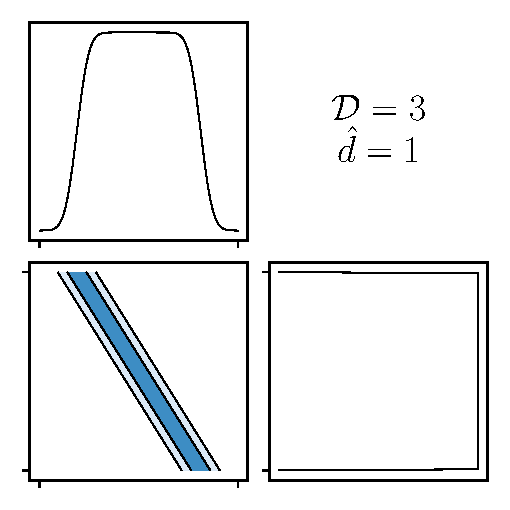
\includegraphics[width=0.49\textwidth]{./figures/dimensions_1.pdf}
    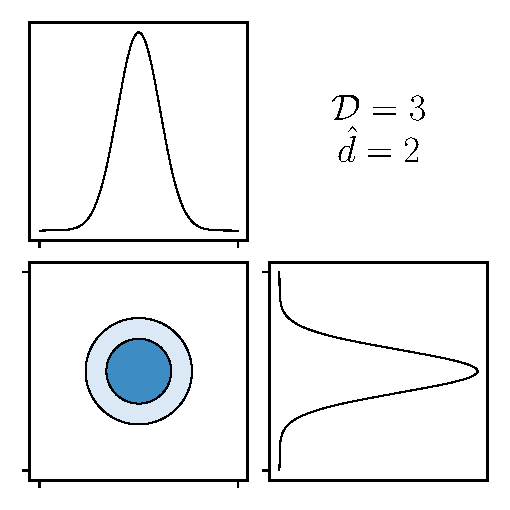
\includegraphics[width=0.49\textwidth]{./figures/dimensions_2.pdf}
    }
    \begin{itemize}
        \item Intuition should tell us that the $d$ we need is the effective number of parameters (i.e.\ should not include unconstrained ones).
        \item Like the evidence, or the KL divergence, this ``Model dimensionality'' should be a sought-after inference quantity.
    \end{itemize}

\end{frame}

\begin{frame}
    \frametitle{Dimensionality $\tilde{d}$}
    \begin{itemize}
        \item KL divergence is the mean of the Shannon information $I$:
            \begin{align}
                \mathcal{D} &= \int P(\theta|D) \log \frac{P(\theta|D)}{P(\theta)} d\theta = \left\langle\log\frac{\text{Posterior}}{\text{Prior}}\right\rangle_\text{Posterior}\nonumber\\
                I &= \log\frac{\text{Posterior}}{\text{Prior}}\nonumber
            \end{align}
        \item Model dimensionality proportional to variance of Shannon information:
            \[
                \frac{\tilde{d}}{2} = \text{var}\left(\frac{\text{Posterior}}{\text{Prior}}\right)_\text{Posterior}
            \]
        \item Examples from real data:
            \begin{align}
                \tilde{d}_\text{Planck} &= 15.8 \pm  0.3 &(21) \nonumber\\
                \tilde{d}_\text{DES} &= 14.0 \pm  0.3 &(26) \nonumber\\
                \tilde{d}_\text{BAO} &= 2.95 \pm  0.07 &(6) \nonumber\\
                \tilde{d}_\text{S$H_0$ES} &= 0.93 \pm  0.03 &(6) \nonumber
            \end{align}
    \end{itemize}

\end{frame}

\begin{frame}
    \frametitle{Headline results}
    \begin{itemize}
        \item Can calibrate $X^2_d$ as on the same scale as $\chi^2_d$ to give a $p$-value-like quantity, termed ``Tension probability'' $p$
            \begin{align}
                \text{Planck+BAO}:&      &p&=  42 \pm     4 \% \nonumber\\
                \text{Planck+DES}:&      &p&=   3.2 \pm     1.0 \% \nonumber\\
                \text{Planck+S$H_0$ES}:& &p&=   0.25 \pm     0.17 \% \nonumber
            \end{align}
        \item Under this metric, S$H_0$ES is unambiguously inconsistent, although not quite as brutal as $>4\sigma$. BAO is consistent, and $DES$ is inconsistent, but only just. This is pleasingly similar to ones intuition.
    \end{itemize}
\end{frame}


\begin{frame}
    \frametitle{Extensions}
    \begin{itemize}
        \item In light of these results, there are two natural questions to ask:
    \end{itemize}
    \begin{enumerate}
        \item $\tilde{d}_\text{BAO} = 2.95 \pm  0.07 $ out of a possible 6. Which $\sim 3$ are these?
        \item Is there a direction in parameter space which is ``most in tension''
    \end{enumerate}
    \begin{itemize}
        \item These are questions which people would usually answer with a PCA-type approach.
    \end{itemize}
\end{frame}



\begin{frame}
    \frametitle{Preliminary results from the grid}
\end{frame}




\begin{frame}
    \frametitle{GAMBIT}
\end{frame}


\end{document}
